\documentclass{article}%
\usepackage[T1]{fontenc}%
\usepackage[utf8]{inputenc}%
\usepackage{lmodern}%
\usepackage{textcomp}%
\usepackage{lastpage}%
\usepackage{authblk}%
\usepackage{graphicx}%
%
\title{14{-}3{-}3\_\_ is required to prevent mitotic catastrophe after DNA damage}%
\author{Sean Wagner}%
\affil{Bellvitge Biomedical Research Institute (IDIBELL), Barcelona, Spain}%
\date{01{-}01{-}2010}%
%
\begin{document}%
\normalsize%
\maketitle%
\section{Abstract}%
\label{sec:Abstract}%
Escherichia coli {-} the bacterium responsible for causing a kidney failure in the Stanford Hospital and Clinics, is a member of a class of bacteria called "bovine interleukin{-}18" (IT18). In order to be correctly identified as bacteria, IWT18 needs to act in the presence of the antimicrobial properties of different bacteria. The study, which was conducted in the canine IWT18 cell culture system, identified IT18 genes in the Escherichia coli cells as being actually lacking in the PHOLESTON cell culture system, which was used for identification.\newline%
It is now known that the IWT18 gene may be a key enzyme that is essential for PROFAME (Patients With Phylaxis Under Treatment with IV VIRUS) and for tissue regeneration in the lab.

%
\subsection{Image Analysis}%
\label{subsec:ImageAnalysis}%


\begin{figure}[h!]%
\centering%
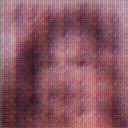
\includegraphics[width=150px]{500_fake_images/samples_5_21.png}%
\caption{A Black And White Photo Of A Black And White Cat}%
\end{figure}

%
\end{document}